% Created by tikzDevice version 0.10.1 on 2016-08-29 22:52:14
% !TEX encoding = UTF-8 Unicode
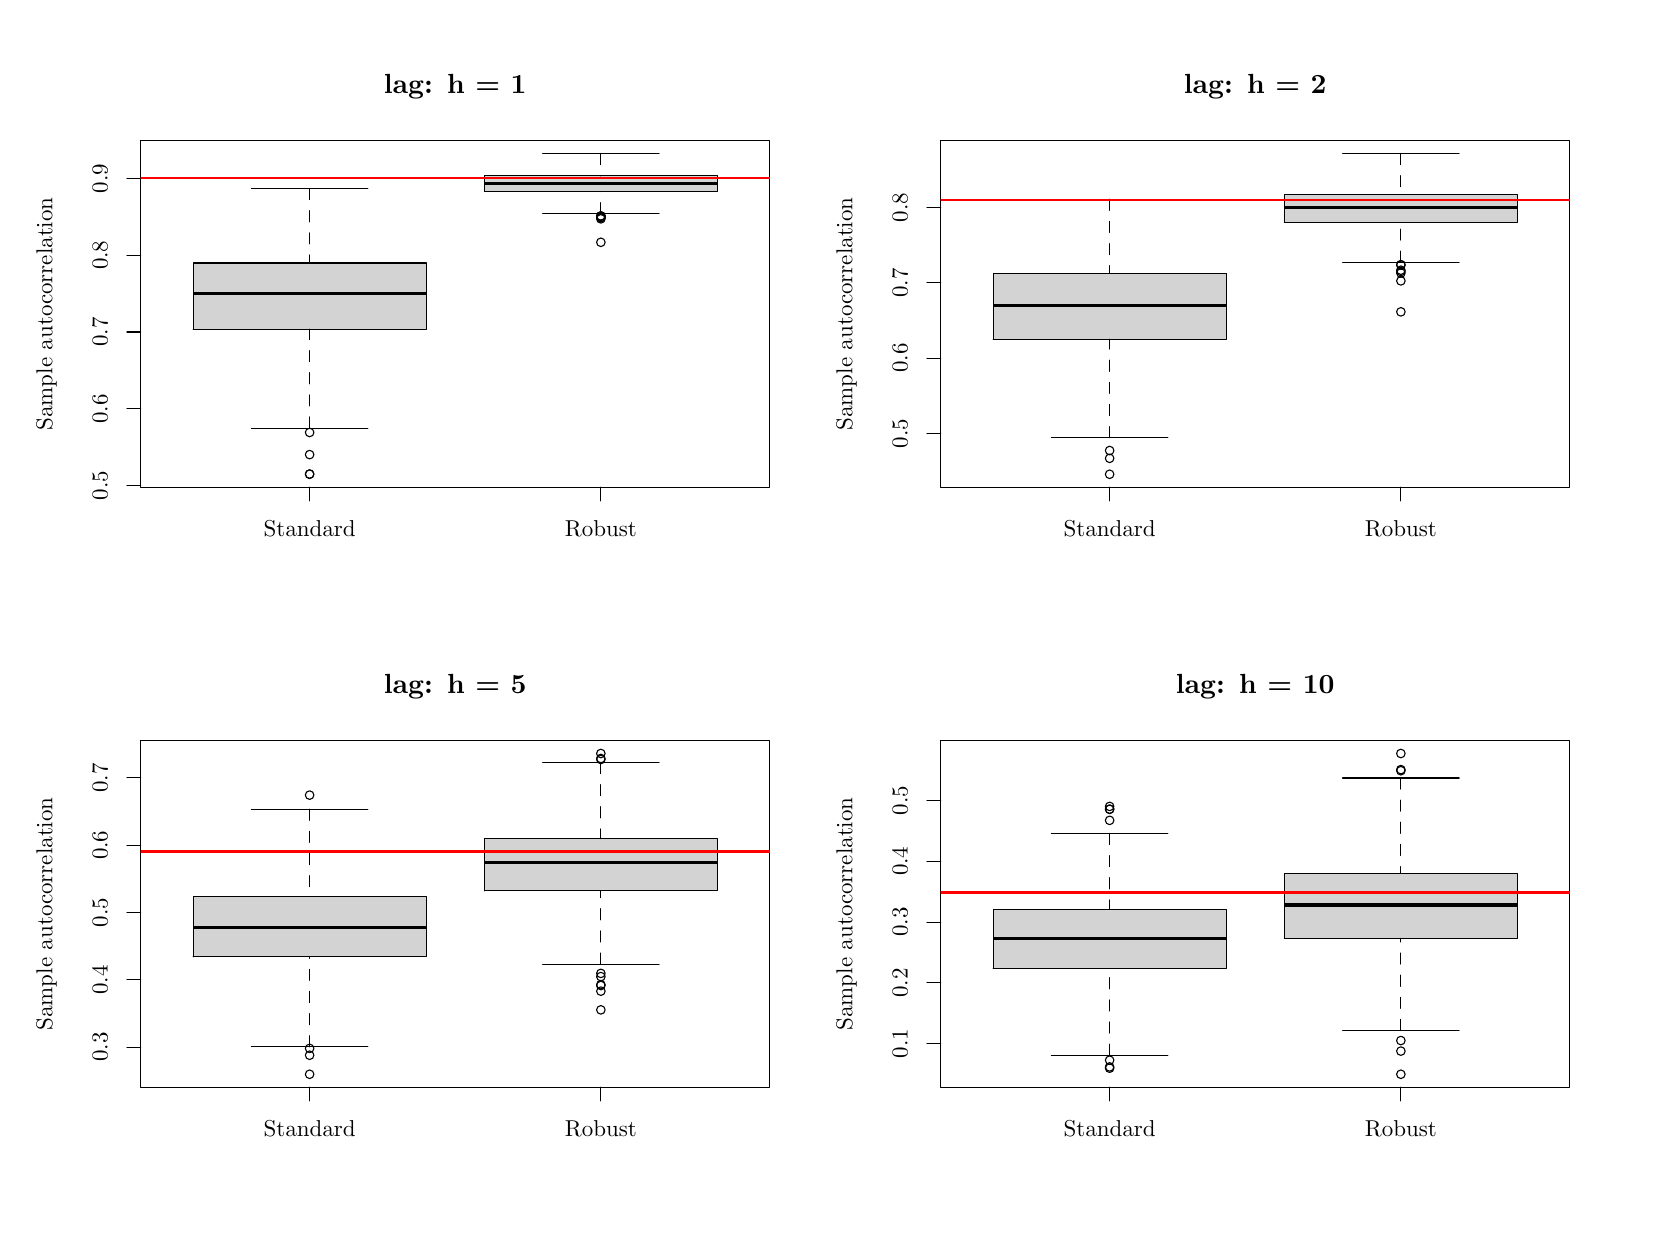
\begin{tikzpicture}[x=1pt,y=1pt]
\definecolor{fillColor}{RGB}{255,255,255}
\path[use as bounding box,fill=fillColor,fill opacity=0.00] (0,0) rectangle (578.16,433.62);
\begin{scope}
\path[clip] ( 40.84,267.61) rectangle (268.16,392.78);
\definecolor{fillColor}{RGB}{211,211,211}

\path[fill=fillColor] ( 59.78,324.66) --
	(143.98,324.66) --
	(143.98,348.59) --
	( 59.78,348.59) --
	cycle;
\definecolor{drawColor}{RGB}{0,0,0}

\path[draw=drawColor,line width= 1.2pt,line join=round] ( 59.78,337.50) -- (143.98,337.50);

\path[draw=drawColor,line width= 0.4pt,dash pattern=on 4pt off 4pt ,line join=round,line cap=round] (101.88,288.93) -- (101.88,324.66);

\path[draw=drawColor,line width= 0.4pt,dash pattern=on 4pt off 4pt ,line join=round,line cap=round] (101.88,375.48) -- (101.88,348.59);

\path[draw=drawColor,line width= 0.4pt,line join=round,line cap=round] ( 80.83,288.93) -- (122.93,288.93);

\path[draw=drawColor,line width= 0.4pt,line join=round,line cap=round] ( 80.83,375.48) -- (122.93,375.48);

\path[draw=drawColor,line width= 0.4pt,line join=round,line cap=round] ( 59.78,324.66) --
	(143.98,324.66) --
	(143.98,348.59) --
	( 59.78,348.59) --
	( 59.78,324.66);

\path[draw=drawColor,line width= 0.4pt,line join=round,line cap=round] (101.88,279.35) circle (  1.55);

\path[draw=drawColor,line width= 0.4pt,line join=round,line cap=round] (101.88,272.24) circle (  1.55);

\path[draw=drawColor,line width= 0.4pt,line join=round,line cap=round] (101.88,287.34) circle (  1.55);

\path[draw=drawColor,line width= 0.4pt,line join=round,line cap=round] (101.88,272.33) circle (  1.55);

\path[fill=fillColor] (165.02,374.47) --
	(249.22,374.47) --
	(249.22,380.09) --
	(165.02,380.09) --
	cycle;

\path[draw=drawColor,line width= 1.2pt,line join=round] (165.02,377.31) -- (249.22,377.31);

\path[draw=drawColor,line width= 0.4pt,dash pattern=on 4pt off 4pt ,line join=round,line cap=round] (207.12,366.38) -- (207.12,374.47);

\path[draw=drawColor,line width= 0.4pt,dash pattern=on 4pt off 4pt ,line join=round,line cap=round] (207.12,388.15) -- (207.12,380.09);

\path[draw=drawColor,line width= 0.4pt,line join=round,line cap=round] (186.07,366.38) -- (228.17,366.38);

\path[draw=drawColor,line width= 0.4pt,line join=round,line cap=round] (186.07,388.15) -- (228.17,388.15);

\path[draw=drawColor,line width= 0.4pt,line join=round,line cap=round] (165.02,374.47) --
	(249.22,374.47) --
	(249.22,380.09) --
	(165.02,380.09) --
	(165.02,374.47);

\path[draw=drawColor,line width= 0.4pt,line join=round,line cap=round] (207.12,365.45) circle (  1.55);

\path[draw=drawColor,line width= 0.4pt,line join=round,line cap=round] (207.12,364.54) circle (  1.55);

\path[draw=drawColor,line width= 0.4pt,line join=round,line cap=round] (207.12,364.90) circle (  1.55);

\path[draw=drawColor,line width= 0.4pt,line join=round,line cap=round] (207.12,356.06) circle (  1.55);

\path[draw=drawColor,line width= 0.4pt,line join=round,line cap=round] (207.12,365.03) circle (  1.55);

\path[draw=drawColor,line width= 0.4pt,line join=round,line cap=round] (207.12,365.54) circle (  1.55);

\path[draw=drawColor,line width= 0.4pt,line join=round,line cap=round] (207.12,365.59) circle (  1.55);
\end{scope}
\begin{scope}
\path[clip] (  0.00,  0.00) rectangle (578.16,433.62);
\definecolor{drawColor}{RGB}{0,0,0}

\path[draw=drawColor,line width= 0.4pt,line join=round,line cap=round] (101.88,267.61) -- (207.12,267.61);

\path[draw=drawColor,line width= 0.4pt,line join=round,line cap=round] (101.88,267.61) -- (101.88,262.63);

\path[draw=drawColor,line width= 0.4pt,line join=round,line cap=round] (207.12,267.61) -- (207.12,262.63);

\node[text=drawColor,anchor=base,inner sep=0pt, outer sep=0pt, scale=  0.83] at (101.88,249.68) {Standard};

\node[text=drawColor,anchor=base,inner sep=0pt, outer sep=0pt, scale=  0.83] at (207.12,249.68) {Robust};

\path[draw=drawColor,line width= 0.4pt,line join=round,line cap=round] ( 40.84,268.13) -- ( 40.84,379.16);

\path[draw=drawColor,line width= 0.4pt,line join=round,line cap=round] ( 40.84,268.13) -- ( 35.86,268.13);

\path[draw=drawColor,line width= 0.4pt,line join=round,line cap=round] ( 40.84,295.89) -- ( 35.86,295.89);

\path[draw=drawColor,line width= 0.4pt,line join=round,line cap=round] ( 40.84,323.64) -- ( 35.86,323.64);

\path[draw=drawColor,line width= 0.4pt,line join=round,line cap=round] ( 40.84,351.40) -- ( 35.86,351.40);

\path[draw=drawColor,line width= 0.4pt,line join=round,line cap=round] ( 40.84,379.16) -- ( 35.86,379.16);

\node[text=drawColor,rotate= 90.00,anchor=base,inner sep=0pt, outer sep=0pt, scale=  0.83] at ( 28.88,268.13) {0.5};

\node[text=drawColor,rotate= 90.00,anchor=base,inner sep=0pt, outer sep=0pt, scale=  0.83] at ( 28.88,295.89) {0.6};

\node[text=drawColor,rotate= 90.00,anchor=base,inner sep=0pt, outer sep=0pt, scale=  0.83] at ( 28.88,323.64) {0.7};

\node[text=drawColor,rotate= 90.00,anchor=base,inner sep=0pt, outer sep=0pt, scale=  0.83] at ( 28.88,351.40) {0.8};

\node[text=drawColor,rotate= 90.00,anchor=base,inner sep=0pt, outer sep=0pt, scale=  0.83] at ( 28.88,379.16) {0.9};
\end{scope}
\begin{scope}
\path[clip] (  0.00,216.81) rectangle (289.08,433.62);
\definecolor{drawColor}{RGB}{0,0,0}

\node[text=drawColor,anchor=base,inner sep=0pt, outer sep=0pt, scale=  1.00] at (154.50,409.77) {\bfseries lag: h =  1};

\node[text=drawColor,rotate= 90.00,anchor=base,inner sep=0pt, outer sep=0pt, scale=  0.83] at (  8.96,330.19) {Sample autocorrelation};
\end{scope}
\begin{scope}
\path[clip] (  0.00,  0.00) rectangle (578.16,433.62);
\definecolor{drawColor}{RGB}{0,0,0}

\path[draw=drawColor,line width= 0.4pt,line join=round,line cap=round] ( 40.84,267.61) --
	(268.16,267.61) --
	(268.16,392.78) --
	( 40.84,392.78) --
	( 40.84,267.61);
\end{scope}
\begin{scope}
\path[clip] ( 40.84,267.61) rectangle (268.16,392.78);
\definecolor{drawColor}{RGB}{255,0,0}

\path[draw=drawColor,line width= 0.8pt,line join=round,line cap=round] ( 40.84,379.16) -- (268.16,379.16);
\end{scope}
\begin{scope}
\path[clip] (329.92,267.61) rectangle (557.24,392.78);
\definecolor{fillColor}{RGB}{211,211,211}

\path[fill=fillColor] (348.86,321.02) --
	(433.06,321.02) --
	(433.06,344.85) --
	(348.86,344.85) --
	cycle;
\definecolor{drawColor}{RGB}{0,0,0}

\path[draw=drawColor,line width= 1.2pt,line join=round] (348.86,333.30) -- (433.06,333.30);

\path[draw=drawColor,line width= 0.4pt,dash pattern=on 4pt off 4pt ,line join=round,line cap=round] (390.96,285.46) -- (390.96,321.02);

\path[draw=drawColor,line width= 0.4pt,dash pattern=on 4pt off 4pt ,line join=round,line cap=round] (390.96,371.61) -- (390.96,344.85);

\path[draw=drawColor,line width= 0.4pt,line join=round,line cap=round] (369.91,285.46) -- (412.01,285.46);

\path[draw=drawColor,line width= 0.4pt,line join=round,line cap=round] (369.91,371.61) -- (412.01,371.61);

\path[draw=drawColor,line width= 0.4pt,line join=round,line cap=round] (348.86,321.02) --
	(433.06,321.02) --
	(433.06,344.85) --
	(348.86,344.85) --
	(348.86,321.02);

\path[draw=drawColor,line width= 0.4pt,line join=round,line cap=round] (390.96,280.82) circle (  1.55);

\path[draw=drawColor,line width= 0.4pt,line join=round,line cap=round] (390.96,278.00) circle (  1.55);

\path[draw=drawColor,line width= 0.4pt,line join=round,line cap=round] (390.96,272.24) circle (  1.55);

\path[fill=fillColor] (454.10,363.34) --
	(538.30,363.34) --
	(538.30,373.43) --
	(454.10,373.43) --
	cycle;

\path[draw=drawColor,line width= 1.2pt,line join=round] (454.10,368.56) -- (538.30,368.56);

\path[draw=drawColor,line width= 0.4pt,dash pattern=on 4pt off 4pt ,line join=round,line cap=round] (496.20,348.83) -- (496.20,363.34);

\path[draw=drawColor,line width= 0.4pt,dash pattern=on 4pt off 4pt ,line join=round,line cap=round] (496.20,388.15) -- (496.20,373.43);

\path[draw=drawColor,line width= 0.4pt,line join=round,line cap=round] (475.15,348.83) -- (517.25,348.83);

\path[draw=drawColor,line width= 0.4pt,line join=round,line cap=round] (475.15,388.15) -- (517.25,388.15);

\path[draw=drawColor,line width= 0.4pt,line join=round,line cap=round] (454.10,363.34) --
	(538.30,363.34) --
	(538.30,373.43) --
	(454.10,373.43) --
	(454.10,363.34);

\path[draw=drawColor,line width= 0.4pt,line join=round,line cap=round] (496.20,345.98) circle (  1.55);

\path[draw=drawColor,line width= 0.4pt,line join=round,line cap=round] (496.20,347.84) circle (  1.55);

\path[draw=drawColor,line width= 0.4pt,line join=round,line cap=round] (496.20,330.93) circle (  1.55);

\path[draw=drawColor,line width= 0.4pt,line join=round,line cap=round] (496.20,342.12) circle (  1.55);

\path[draw=drawColor,line width= 0.4pt,line join=round,line cap=round] (496.20,347.98) circle (  1.55);

\path[draw=drawColor,line width= 0.4pt,line join=round,line cap=round] (496.20,345.53) circle (  1.55);

\path[draw=drawColor,line width= 0.4pt,line join=round,line cap=round] (496.20,344.94) circle (  1.55);
\end{scope}
\begin{scope}
\path[clip] (  0.00,  0.00) rectangle (578.16,433.62);
\definecolor{drawColor}{RGB}{0,0,0}

\path[draw=drawColor,line width= 0.4pt,line join=round,line cap=round] (390.96,267.61) -- (496.20,267.61);

\path[draw=drawColor,line width= 0.4pt,line join=round,line cap=round] (390.96,267.61) -- (390.96,262.63);

\path[draw=drawColor,line width= 0.4pt,line join=round,line cap=round] (496.20,267.61) -- (496.20,262.63);

\node[text=drawColor,anchor=base,inner sep=0pt, outer sep=0pt, scale=  0.83] at (390.96,249.68) {Standard};

\node[text=drawColor,anchor=base,inner sep=0pt, outer sep=0pt, scale=  0.83] at (496.20,249.68) {Robust};

\path[draw=drawColor,line width= 0.4pt,line join=round,line cap=round] (329.92,287.03) -- (329.92,368.56);

\path[draw=drawColor,line width= 0.4pt,line join=round,line cap=round] (329.92,287.03) -- (324.94,287.03);

\path[draw=drawColor,line width= 0.4pt,line join=round,line cap=round] (329.92,314.21) -- (324.94,314.21);

\path[draw=drawColor,line width= 0.4pt,line join=round,line cap=round] (329.92,341.39) -- (324.94,341.39);

\path[draw=drawColor,line width= 0.4pt,line join=round,line cap=round] (329.92,368.56) -- (324.94,368.56);

\node[text=drawColor,rotate= 90.00,anchor=base,inner sep=0pt, outer sep=0pt, scale=  0.83] at (317.96,287.03) {0.5};

\node[text=drawColor,rotate= 90.00,anchor=base,inner sep=0pt, outer sep=0pt, scale=  0.83] at (317.96,314.21) {0.6};

\node[text=drawColor,rotate= 90.00,anchor=base,inner sep=0pt, outer sep=0pt, scale=  0.83] at (317.96,341.39) {0.7};

\node[text=drawColor,rotate= 90.00,anchor=base,inner sep=0pt, outer sep=0pt, scale=  0.83] at (317.96,368.56) {0.8};
\end{scope}
\begin{scope}
\path[clip] (289.08,216.81) rectangle (578.16,433.62);
\definecolor{drawColor}{RGB}{0,0,0}

\node[text=drawColor,anchor=base,inner sep=0pt, outer sep=0pt, scale=  1.00] at (443.58,409.77) {\bfseries lag: h =  2};

\node[text=drawColor,rotate= 90.00,anchor=base,inner sep=0pt, outer sep=0pt, scale=  0.83] at (298.04,330.19) {Sample autocorrelation};
\end{scope}
\begin{scope}
\path[clip] (  0.00,  0.00) rectangle (578.16,433.62);
\definecolor{drawColor}{RGB}{0,0,0}

\path[draw=drawColor,line width= 0.4pt,line join=round,line cap=round] (329.92,267.61) --
	(557.24,267.61) --
	(557.24,392.78) --
	(329.92,392.78) --
	(329.92,267.61);
\end{scope}
\begin{scope}
\path[clip] (329.92,267.61) rectangle (557.24,392.78);
\definecolor{drawColor}{RGB}{255,0,0}

\path[draw=drawColor,line width= 0.8pt,line join=round,line cap=round] (329.92,371.28) -- (557.24,371.28);
\end{scope}
\begin{scope}
\path[clip] ( 40.84, 50.80) rectangle (268.16,175.97);
\definecolor{fillColor}{RGB}{211,211,211}

\path[fill=fillColor] ( 59.78, 97.88) --
	(143.98, 97.88) --
	(143.98,119.69) --
	( 59.78,119.69) --
	cycle;
\definecolor{drawColor}{RGB}{0,0,0}

\path[draw=drawColor,line width= 1.2pt,line join=round] ( 59.78,108.47) -- (143.98,108.47);

\path[draw=drawColor,line width= 0.4pt,dash pattern=on 4pt off 4pt ,line join=round,line cap=round] (101.88, 65.34) -- (101.88, 97.88);

\path[draw=drawColor,line width= 0.4pt,dash pattern=on 4pt off 4pt ,line join=round,line cap=round] (101.88,151.22) -- (101.88,119.69);

\path[draw=drawColor,line width= 0.4pt,line join=round,line cap=round] ( 80.83, 65.34) -- (122.93, 65.34);

\path[draw=drawColor,line width= 0.4pt,line join=round,line cap=round] ( 80.83,151.22) -- (122.93,151.22);

\path[draw=drawColor,line width= 0.4pt,line join=round,line cap=round] ( 59.78, 97.88) --
	(143.98, 97.88) --
	(143.98,119.69) --
	( 59.78,119.69) --
	( 59.78, 97.88);

\path[draw=drawColor,line width= 0.4pt,line join=round,line cap=round] (101.88, 55.43) circle (  1.55);

\path[draw=drawColor,line width= 0.4pt,line join=round,line cap=round] (101.88, 62.31) circle (  1.55);

\path[draw=drawColor,line width= 0.4pt,line join=round,line cap=round] (101.88, 64.78) circle (  1.55);

\path[draw=drawColor,line width= 0.4pt,line join=round,line cap=round] (101.88,156.30) circle (  1.55);

\path[fill=fillColor] (165.02,121.68) --
	(249.22,121.68) --
	(249.22,140.60) --
	(165.02,140.60) --
	cycle;

\path[draw=drawColor,line width= 1.2pt,line join=round] (165.02,132.01) -- (249.22,132.01);

\path[draw=drawColor,line width= 0.4pt,dash pattern=on 4pt off 4pt ,line join=round,line cap=round] (207.12, 95.24) -- (207.12,121.68);

\path[draw=drawColor,line width= 0.4pt,dash pattern=on 4pt off 4pt ,line join=round,line cap=round] (207.12,168.11) -- (207.12,140.60);

\path[draw=drawColor,line width= 0.4pt,line join=round,line cap=round] (186.07, 95.24) -- (228.17, 95.24);

\path[draw=drawColor,line width= 0.4pt,line join=round,line cap=round] (186.07,168.11) -- (228.17,168.11);

\path[draw=drawColor,line width= 0.4pt,line join=round,line cap=round] (165.02,121.68) --
	(249.22,121.68) --
	(249.22,140.60) --
	(165.02,140.60) --
	(165.02,121.68);

\path[draw=drawColor,line width= 0.4pt,line join=round,line cap=round] (207.12, 91.88) circle (  1.55);

\path[draw=drawColor,line width= 0.4pt,line join=round,line cap=round] (207.12, 90.72) circle (  1.55);

\path[draw=drawColor,line width= 0.4pt,line join=round,line cap=round] (207.12,171.34) circle (  1.55);

\path[draw=drawColor,line width= 0.4pt,line join=round,line cap=round] (207.12, 87.81) circle (  1.55);

\path[draw=drawColor,line width= 0.4pt,line join=round,line cap=round] (207.12, 87.50) circle (  1.55);

\path[draw=drawColor,line width= 0.4pt,line join=round,line cap=round] (207.12, 78.70) circle (  1.55);

\path[draw=drawColor,line width= 0.4pt,line join=round,line cap=round] (207.12,169.53) circle (  1.55);

\path[draw=drawColor,line width= 0.4pt,line join=round,line cap=round] (207.12,169.18) circle (  1.55);

\path[draw=drawColor,line width= 0.4pt,line join=round,line cap=round] (207.12, 85.46) circle (  1.55);
\end{scope}
\begin{scope}
\path[clip] (  0.00,  0.00) rectangle (578.16,433.62);
\definecolor{drawColor}{RGB}{0,0,0}

\path[draw=drawColor,line width= 0.4pt,line join=round,line cap=round] (101.88, 50.80) -- (207.12, 50.80);

\path[draw=drawColor,line width= 0.4pt,line join=round,line cap=round] (101.88, 50.80) -- (101.88, 45.82);

\path[draw=drawColor,line width= 0.4pt,line join=round,line cap=round] (207.12, 50.80) -- (207.12, 45.82);

\node[text=drawColor,anchor=base,inner sep=0pt, outer sep=0pt, scale=  0.83] at (101.88, 32.87) {Standard};

\node[text=drawColor,anchor=base,inner sep=0pt, outer sep=0pt, scale=  0.83] at (207.12, 32.87) {Robust};

\path[draw=drawColor,line width= 0.4pt,line join=round,line cap=round] ( 40.84, 65.24) -- ( 40.84,162.53);

\path[draw=drawColor,line width= 0.4pt,line join=round,line cap=round] ( 40.84, 65.24) -- ( 35.86, 65.24);

\path[draw=drawColor,line width= 0.4pt,line join=round,line cap=round] ( 40.84, 89.56) -- ( 35.86, 89.56);

\path[draw=drawColor,line width= 0.4pt,line join=round,line cap=round] ( 40.84,113.89) -- ( 35.86,113.89);

\path[draw=drawColor,line width= 0.4pt,line join=round,line cap=round] ( 40.84,138.21) -- ( 35.86,138.21);

\path[draw=drawColor,line width= 0.4pt,line join=round,line cap=round] ( 40.84,162.53) -- ( 35.86,162.53);

\node[text=drawColor,rotate= 90.00,anchor=base,inner sep=0pt, outer sep=0pt, scale=  0.83] at ( 28.88, 65.24) {0.3};

\node[text=drawColor,rotate= 90.00,anchor=base,inner sep=0pt, outer sep=0pt, scale=  0.83] at ( 28.88, 89.56) {0.4};

\node[text=drawColor,rotate= 90.00,anchor=base,inner sep=0pt, outer sep=0pt, scale=  0.83] at ( 28.88,113.89) {0.5};

\node[text=drawColor,rotate= 90.00,anchor=base,inner sep=0pt, outer sep=0pt, scale=  0.83] at ( 28.88,138.21) {0.6};

\node[text=drawColor,rotate= 90.00,anchor=base,inner sep=0pt, outer sep=0pt, scale=  0.83] at ( 28.88,162.53) {0.7};
\end{scope}
\begin{scope}
\path[clip] (  0.00,  0.00) rectangle (289.08,216.81);
\definecolor{drawColor}{RGB}{0,0,0}

\node[text=drawColor,anchor=base,inner sep=0pt, outer sep=0pt, scale=  1.00] at (154.50,192.96) {\bfseries lag: h =  5};

\node[text=drawColor,rotate= 90.00,anchor=base,inner sep=0pt, outer sep=0pt, scale=  0.83] at (  8.96,113.38) {Sample autocorrelation};
\end{scope}
\begin{scope}
\path[clip] (  0.00,  0.00) rectangle (578.16,433.62);
\definecolor{drawColor}{RGB}{0,0,0}

\path[draw=drawColor,line width= 0.4pt,line join=round,line cap=round] ( 40.84, 50.80) --
	(268.16, 50.80) --
	(268.16,175.97) --
	( 40.84,175.97) --
	( 40.84, 50.80);
\end{scope}
\begin{scope}
\path[clip] ( 40.84, 50.80) rectangle (268.16,175.97);
\definecolor{drawColor}{RGB}{255,0,0}

\path[draw=drawColor,line width= 0.8pt,line join=round,line cap=round] ( 40.84,135.90) -- (268.16,135.90);
\end{scope}
\begin{scope}
\path[clip] (329.92, 50.80) rectangle (557.24,175.97);
\definecolor{fillColor}{RGB}{211,211,211}

\path[fill=fillColor] (348.86, 93.72) --
	(433.06, 93.72) --
	(433.06,115.09) --
	(348.86,115.09) --
	cycle;
\definecolor{drawColor}{RGB}{0,0,0}

\path[draw=drawColor,line width= 1.2pt,line join=round] (348.86,104.50) -- (433.06,104.50);

\path[draw=drawColor,line width= 0.4pt,dash pattern=on 4pt off 4pt ,line join=round,line cap=round] (390.96, 62.31) -- (390.96, 93.72);

\path[draw=drawColor,line width= 0.4pt,dash pattern=on 4pt off 4pt ,line join=round,line cap=round] (390.96,142.46) -- (390.96,115.09);

\path[draw=drawColor,line width= 0.4pt,line join=round,line cap=round] (369.91, 62.31) -- (412.01, 62.31);

\path[draw=drawColor,line width= 0.4pt,line join=round,line cap=round] (369.91,142.46) -- (412.01,142.46);

\path[draw=drawColor,line width= 0.4pt,line join=round,line cap=round] (348.86, 93.72) --
	(433.06, 93.72) --
	(433.06,115.09) --
	(348.86,115.09) --
	(348.86, 93.72);

\path[draw=drawColor,line width= 0.4pt,line join=round,line cap=round] (390.96,151.24) circle (  1.55);

\path[draw=drawColor,line width= 0.4pt,line join=round,line cap=round] (390.96, 60.51) circle (  1.55);

\path[draw=drawColor,line width= 0.4pt,line join=round,line cap=round] (390.96,151.17) circle (  1.55);

\path[draw=drawColor,line width= 0.4pt,line join=round,line cap=round] (390.96, 58.10) circle (  1.55);

\path[draw=drawColor,line width= 0.4pt,line join=round,line cap=round] (390.96, 57.63) circle (  1.55);

\path[draw=drawColor,line width= 0.4pt,line join=round,line cap=round] (390.96,152.22) circle (  1.55);

\path[draw=drawColor,line width= 0.4pt,line join=round,line cap=round] (390.96,147.18) circle (  1.55);

\path[fill=fillColor] (454.10,104.55) --
	(538.30,104.55) --
	(538.30,128.08) --
	(454.10,128.08) --
	cycle;

\path[draw=drawColor,line width= 1.2pt,line join=round] (454.10,116.55) -- (538.30,116.55);

\path[draw=drawColor,line width= 0.4pt,dash pattern=on 4pt off 4pt ,line join=round,line cap=round] (496.20, 71.24) -- (496.20,104.55);

\path[draw=drawColor,line width= 0.4pt,dash pattern=on 4pt off 4pt ,line join=round,line cap=round] (496.20,162.49) -- (496.20,128.08);

\path[draw=drawColor,line width= 0.4pt,line join=round,line cap=round] (475.15, 71.24) -- (517.25, 71.24);

\path[draw=drawColor,line width= 0.4pt,line join=round,line cap=round] (475.15,162.49) -- (517.25,162.49);

\path[draw=drawColor,line width= 0.4pt,line join=round,line cap=round] (454.10,104.55) --
	(538.30,104.55) --
	(538.30,128.08) --
	(454.10,128.08) --
	(454.10,104.55);

\path[draw=drawColor,line width= 0.4pt,line join=round,line cap=round] (496.20, 63.80) circle (  1.55);

\path[draw=drawColor,line width= 0.4pt,line join=round,line cap=round] (496.20,165.12) circle (  1.55);

\path[draw=drawColor,line width= 0.4pt,line join=round,line cap=round] (496.20, 55.43) circle (  1.55);

\path[draw=drawColor,line width= 0.4pt,line join=round,line cap=round] (496.20,171.34) circle (  1.55);

\path[draw=drawColor,line width= 0.4pt,line join=round,line cap=round] (496.20,165.52) circle (  1.55);

\path[draw=drawColor,line width= 0.4pt,line join=round,line cap=round] (496.20, 67.61) circle (  1.55);
\end{scope}
\begin{scope}
\path[clip] (  0.00,  0.00) rectangle (578.16,433.62);
\definecolor{drawColor}{RGB}{0,0,0}

\path[draw=drawColor,line width= 0.4pt,line join=round,line cap=round] (390.96, 50.80) -- (496.20, 50.80);

\path[draw=drawColor,line width= 0.4pt,line join=round,line cap=round] (390.96, 50.80) -- (390.96, 45.82);

\path[draw=drawColor,line width= 0.4pt,line join=round,line cap=round] (496.20, 50.80) -- (496.20, 45.82);

\node[text=drawColor,anchor=base,inner sep=0pt, outer sep=0pt, scale=  0.83] at (390.96, 32.87) {Standard};

\node[text=drawColor,anchor=base,inner sep=0pt, outer sep=0pt, scale=  0.83] at (496.20, 32.87) {Robust};

\path[draw=drawColor,line width= 0.4pt,line join=round,line cap=round] (329.92, 66.50) -- (329.92,154.34);

\path[draw=drawColor,line width= 0.4pt,line join=round,line cap=round] (329.92, 66.50) -- (324.94, 66.50);

\path[draw=drawColor,line width= 0.4pt,line join=round,line cap=round] (329.92, 88.46) -- (324.94, 88.46);

\path[draw=drawColor,line width= 0.4pt,line join=round,line cap=round] (329.92,110.42) -- (324.94,110.42);

\path[draw=drawColor,line width= 0.4pt,line join=round,line cap=round] (329.92,132.38) -- (324.94,132.38);

\path[draw=drawColor,line width= 0.4pt,line join=round,line cap=round] (329.92,154.34) -- (324.94,154.34);

\node[text=drawColor,rotate= 90.00,anchor=base,inner sep=0pt, outer sep=0pt, scale=  0.83] at (317.96, 66.50) {0.1};

\node[text=drawColor,rotate= 90.00,anchor=base,inner sep=0pt, outer sep=0pt, scale=  0.83] at (317.96, 88.46) {0.2};

\node[text=drawColor,rotate= 90.00,anchor=base,inner sep=0pt, outer sep=0pt, scale=  0.83] at (317.96,110.42) {0.3};

\node[text=drawColor,rotate= 90.00,anchor=base,inner sep=0pt, outer sep=0pt, scale=  0.83] at (317.96,132.38) {0.4};

\node[text=drawColor,rotate= 90.00,anchor=base,inner sep=0pt, outer sep=0pt, scale=  0.83] at (317.96,154.34) {0.5};
\end{scope}
\begin{scope}
\path[clip] (289.08,  0.00) rectangle (578.16,216.81);
\definecolor{drawColor}{RGB}{0,0,0}

\node[text=drawColor,anchor=base,inner sep=0pt, outer sep=0pt, scale=  1.00] at (443.58,192.96) {\bfseries lag: h =  10};

\node[text=drawColor,rotate= 90.00,anchor=base,inner sep=0pt, outer sep=0pt, scale=  0.83] at (298.04,113.38) {Sample autocorrelation};
\end{scope}
\begin{scope}
\path[clip] (  0.00,  0.00) rectangle (578.16,433.62);
\definecolor{drawColor}{RGB}{0,0,0}

\path[draw=drawColor,line width= 0.4pt,line join=round,line cap=round] (329.92, 50.80) --
	(557.24, 50.80) --
	(557.24,175.97) --
	(329.92,175.97) --
	(329.92, 50.80);
\end{scope}
\begin{scope}
\path[clip] (329.92, 50.80) rectangle (557.24,175.97);
\definecolor{drawColor}{RGB}{255,0,0}

\path[draw=drawColor,line width= 0.8pt,line join=round,line cap=round] (329.92,121.11) -- (557.24,121.11);
\end{scope}
\end{tikzpicture}
